\chapter{State of the Art}
%What was given to me
The current moduro project has a stable 2D simulation of 16 different models using \ac{CC3D}. With these models it is tried to make predictions about how bladder cancer arises. The simulations are performed by \ac{CC3D} and then several values, e.g. the fitness of the model or how realistic the model is, etc., are summarized and displayed by the 'Moduro-Toolbox'. The project consits of several models and several scripts, both are written in python, i.e. a programming language. The models include properties of the specific model, e.g. adhesion energy or the possibility of the new cell types after mitosis, i.e. cell division, and the scripts modify the cell behavior, e.g. they check when a mitosis takes place, how fast the cell will growth, etc.. The scripts are also calculating if the current model is a realistic one or not. These evaluating data are later used by the 'Moduro-Toolbox' to provide a overview over these data.

\section{Display and Simulation of the Urothelium}
%wie wird es dargestellt 
In \ac{CC3D} we simulate an urothel of the size of \SI{333}{\micro\metre} for the x-axis and \SI{100}{\micro\metre} for the y-axis. Because, \ac{CC3D} has its constraints about the size if we use only one core of the prozessor the size of the simulation will be rescaled to its maximum limitations of \SI{267}{\micro\metre} for the x-axis and \SI{80}{\micro\metre} for the y-axis in two dimensions. \newline 
The simulation of the urothel covers 720 days. At the first calculation step, \ac{MCS} 0, the simulation is initialized, i.e. the cells are drawn and placed on the basal membrane. A illustration of an initial simulation is displayed in figure \ref{img:2DSimulationInitialState} at page \pageref{img:2DSimulationInitialState}. Since we simulate morphogenesis, the urothelium is proposed to growth and to proliferate in the given area. An illustration therefor is presented in figure \ref{img:2DSimulation33Days} at page \pageref{img:2DSimulation33Days}. \newline
In order to provide a realistic simulation, the simulation has to be not to easy and not to hard, we have to simulate events which occur every \ac{MCS} and some events which are occur not every \ac{MCS}. The events, which are performed every \ac{MCS} are a) cell growth and b) the check for mitosis. Events which are not performed every \ac{MCS} are c) urination d) cell death e) cell transformation and f) cell mutation. These events are presented in detail in the following.

\begin{figure}
	\center
	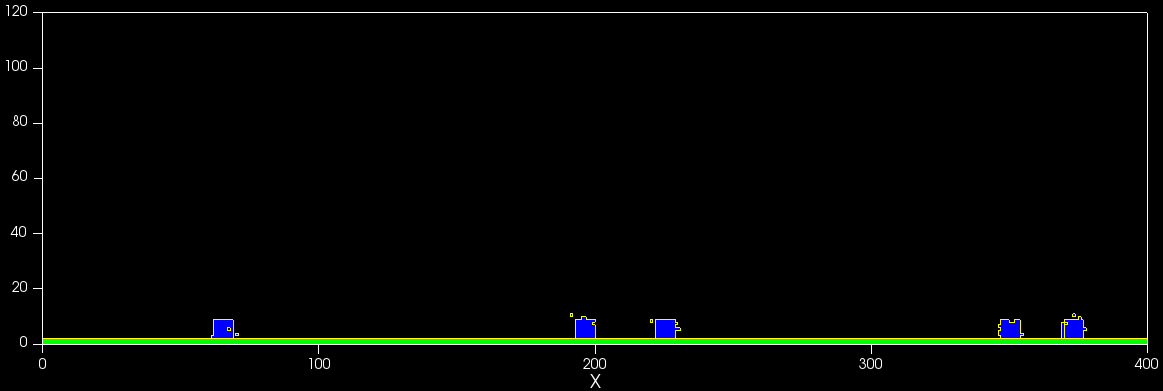
\includegraphics[scale=0.35]{figures/2DSimulation-InitialState.png}
	\caption{Initial state of an 2D simulation}
	\label{img:2DSimulationInitialState}
\end{figure}

\begin{figure}
	\center
	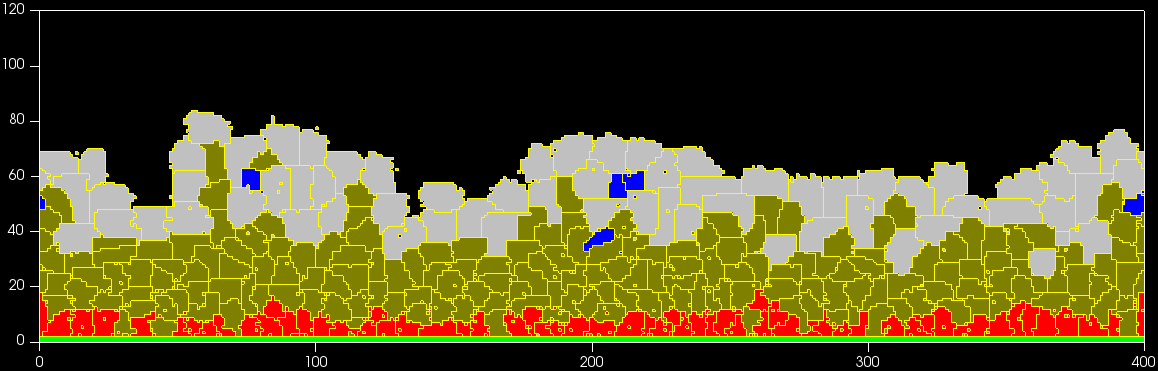
\includegraphics[scale=0.35]{figures/2DSimulation-33Days.png}
	\caption{2D Simulation after 33 days}
	\label{img:2DSimulation33Days}
\end{figure}

\subsection{Events in the simulation}
In this subsection the events for the simulation are presented. All of these events are executed every \ac{MCS}, excluding the initializing step, \ac{MCS} 0, and every factor of 250, \ac{MCS} 250, 500, 750, etc.. \newline
The urination takes place every 12 hours, it should be simulated every 6 hours but because these events are not called every 250 \ac{MCS}, it is only called every 12 hours.

\subsubsection{Cell Growth}
Every \ac{MCS} we calculate the growth of a cell. In the project the maximum possible growth of a cell is calculated and applied.  We need this calculation for the relation volume and target volume as well as for the relation volume, surface and target surface. Since, the volume and the surface of a cell is calculated by \ac{CC3D}. The only way to influence it, is by setting the correct $\lambda$ values, for the volume and surface, and by additional calculating the target volume and target surface values. In the program the calculation of the target volume and the target surface, i.e. the volume and surface which the cell should have, is made. \ac{CC3D} uses the lambda mulitplier and the target values to calculate the effective energy. Of this calculated energy it is able to calculate the volume and the surface of each cell. This is why we calculate the target volume and surface instead of the actual volume and surface of a cell.

\subsubsection{Mitosis}
The verification if a cell divides or growth further is done in every simulation step. Doing so allows us to define a very specific \ac{MCS} at which a cell divides, as there a 500 \ac{MCS} per day. In order that a cell divides it needs to growth over its maximal size before it divides.
The cells which are able to growth and as a result divide are a) stem cells b) basal cells and c)intermediate cells. 

The umbrella cells are a product of mitosis than of cell division, if they would divide there would be two instead of one umbrella cell.

\subsubsection{Necrosis}
If a cell dies necrosis takes place. In the program a flag in the cell dictionary is set. Every \ac{MCS}, the program checks if a cell dies or not. If so, the cell will shrink and as a result dissappear.

\subsubsection{Mutation}
After 2 days, 1000\ac{MCS}, it is possible that a cell mutates, i.e. it becomes evil. We simulate the possibility for cells to mutate after 2 days, because otherwise there would not be much cells around the mutated cell. Each cell type has its own propability to become evil, in the current simulation it is not considered that cells mutate since the propability for each cell type to mutate is 0\%. \newline
If a cell mutates, there is also the flag for necrosis set. Thus, the cell shrinks and dissappears.


\subsubsection{Transformation}
A transformation can take place if a basal cell divides into a basal and a intermediate cell. Because the intermediate cell has to be inside the strata, it immediately will be transformed to an umbrella cell, which are kind the barrier to the urin in the bladder. 


\subsubsection{Urination}
Every 12 hours an urination takes place. This is simulated in a way that randomly 2\% of the cells in direct contact with the bladder are washed out \cite{Torelli2017}. In the program a flag for necrosis is set and the cells will dissappear because of the necrosis event.








\section{Models}
The 2D simulation of the urothel provided 16 different models. These model differ mostly in which cell types after the mitosis are created. The project divides the models into two domains, one has the id 'SSD', which stands for "stem cell-like division" \cite{Torelli2017} and means that every time a stem cell divides there will be one stem and one basal cell. The second domain has the id 'SPA', which stands for "stem cell population asymmetry" \cite{Torelli2017}. In the second domain the stem cell has a propability of 90\% that it will be one stem and one basal cells after mitosis. There is also the chance with a probability of 5\% that after mitosis of a stem cell there are two stem cells or two basal cells. \newline
For the mitosis of basal cells there are 4 different models. The first one, 'BSD', describes the each basal cell which undergoes mitosis will create one basal and one intermediate cell. The second model describes that there is a 5\% chance that the basal cell will become two basal or two intermediate cells. There is a 90\% propability that the cell become one basal and one intermediate cell. The third model 'BPCD', describes that always a basal cells becomes two basal cells during mitosis and if the basal cell is not on the basal membrane it transform into an intermediate cell. The last model of the basal cells is the 'BCD'. In this model the basal cells immediately transform into an intermediate cell if it is not at the basal membrane anymore.\newline
There are two different models how intermediate cell divide. One is the 'IPCD', a intermediate cell becomes always into two intermediate cells during mitosis and if there is no cell around the specific cell it will be transformed into an umbrella cell. The second one is the 'ICD', in this one only transformation of the intermediate cells into the umbrella cells happens. \newline
With these different proliferation concepts there are 16 models in the project overall. These models were created by an earlier version of the project \cite{Torellie2017} and are displayed in table \ref{tbl:16Models} at page \pageref{tbl:16Models}.


\begin{table}
\begin{centering}
\par\end{centering}
\begin{centering}
\begin{tabularx}{\textwidth}{|c|c|Xc|}
\hline 
Type & ID & Description & Model\tabularnewline
\hline 
\hline 
\multirow{2}{0.02\textwidth}{\begin{turn}{90}
Stem cells
\end{turn}} & SSD & Stem cell-like division & \begin{tikzpicture}[]
\node[SType] {S} [grow=right]
	child {node [SType]  {S}
	}
	child {node [BType]  {B}
	};
\end{tikzpicture}\tabularnewline
\cline{2-4} 
 & SPA & Stem cell population asymmetry & \begin{tikzpicture}[]
\node[SType] {S} [grow=right]
	child {node [SType]  {S}
	}
	child {node [SType]  {S}
	};
\node at (0.5,-1) {$p_s=0.05$};
\node[SType] at (2,0) {S} [grow=right]
	child {node [SType]  {S}
	}
	child {node [BType]  {B}
	};    
\node at (2.5,-1) {$p_a=0.90$};    
\node[SType] at (4,0) {S} [grow=right]
	child {node [BType]  {B}
	}
	child {node [BType]  {B}
	};    
\node at (4.5,-1) {$p_s=0.05$};        
\end{tikzpicture}
\tabularnewline
\hline 
\multirow{4}{0.02\textwidth}{\begin{turn}{90}
Basal cells\ \ \ \ \ \ \ \ \ \ \ \ \ \ \ \ \ \ \ \
\end{turn}} & BSD & Stem cell-like division in basal cell & 
\begin{tikzpicture}[]
\node[BType] {B} [grow=right]
	child {node [IType]  {I}
	}
	child {node [BType]  {B}
	};
\end{tikzpicture}
\tabularnewline
\cline{2-4} 
 & BPA & Basal cell population asymmetry & \begin{tikzpicture}[]
\node[BType] {B} [grow=right]
	child {node [BType]  {B}
	}
	child {node [BType]  {B}
	};
\node at (0.5,-1) {$p_s=0.05$};
\node[BType] at (2,0) {B} [grow=right]
	child {node [BType]  {B}
	}
	child {node [IType]  {I}
	};    
\node at (2.5,-1) {$p_a=0.90$};    
\node[BType] at (4,0) {B} [grow=right]
	child {node [IType]  {I}
	}
	child {node [IType]  {I}
	};    
\node at (4.5,-1) {$p_s=0.05$};        
\end{tikzpicture}\tabularnewline
\cline{2-4} 
 & BPCD & Proliferation and contact differentiation of basal cells & \begin{tikzpicture}[]
\node[BType] {B} [grow=right]
	child {node [BType]  {B}
	}
	child {node [BType]  {B}
	};
\end{tikzpicture} \hspace{1em} and \hspace{1em}
\begin{tikzpicture}[]
\node[BType] {B} [grow=right]
	child[dashed] {node [IType] {I} edge from parent node[above=0.4cm] {$\neg$ BM}
	};
\end{tikzpicture}\tabularnewline
\cline{2-4} 
 & BCD & Only contact differentiation of basal cells & 
\begin{tikzpicture}[]
\node[BType] {B} [grow=right]
	child[dashed] {node [IType] {I} edge from parent node[above=0.4cm] {$\neg$ BM}
	};
\end{tikzpicture}\tabularnewline
\hline 
\multirow{2}{0.02\textwidth}{\begin{turn}{90}
Intermediate cells
\end{turn}} & IPCD & Proliferation and contact differentiation of intermediate cells & \begin{tikzpicture}[]
\node[IType] {I} [grow=right]
	child {node [IType]  {I}
	}
	child {node [IType]  {I}
	};
\end{tikzpicture} \hspace{1em} and \hspace{1em}
\begin{tikzpicture}[]
\node[IType] {I} [grow=right]
	child[dashed] {node [UType] {U} edge from parent node[above=0.4cm] {M}
	};
\end{tikzpicture}
\tabularnewline
\cline{2-4} 
 & ICD & Only contact differentiation of intermediate cells & 
\begin{tikzpicture}[]
\node[IType] {I} [grow=right]
	child[dashed] {node [UType] {U} edge from parent node[above=0.4cm] {M}
	};
\end{tikzpicture}
\tabularnewline
\hline 
\end{tabularx}
\par\end{centering}
\caption{\label{tbl:16Models}16 different models derived in the project as there are different ways of proliferation and mitosis are simulated for the different cell types.}
\end{table}

\section{Adhesion and cell sorting}
During morphogensis of a strata the cells not only growth, they also sort themself. In order for the cell sorting there have to be different adhesion values \cite{REF}, i.e. how strong the surface of two different cell types are holding together. In the project this is done with a matrix, which every of the 16 model has. Such a matrix was created in an earlier version of the project \cite{Torelli2017} and is displayed in table \ref{tbl:AdhesionMatrix} at page \pageref{tbl:AdhesionMatrix}. In this table small values refer to more adhesion wheras larger values refer to less adhesion. The adhesion is calculated by \ac{CC3D}. The cell type 'Medium' is a \ac{CC3D} specific cell type and describe the space where no cells are in the simulation.

\begin{table}
\begin{centering}
\begin{tabular}{|c|c||c|c|c|c|c|c|}
\hline 
\multicolumn{2}{|c||}{Types} & M & BM & \celltypeS & \celltypeB & \celltypeI & \celltypeU \tabularnewline
\hline 
\hline 
Medium & M & 0 & 14 & 14 & 14 & 14 & 4\tabularnewline
\hline 
Basal membrane & BM &  & -1 & 1 & 3 & 12 & 12\tabularnewline
\hline 
Stem cell & \celltypeS &  &  & 6 & 4 & 8 & 14\tabularnewline
\hline 
Basal cell & \celltypeB &  &  &  & 5 & 8 & 12\tabularnewline
\hline 
Intermediate cell & \celltypeI &  &  &  &  & 6 & 4\tabularnewline
\hline 
Umbrella cell & \celltypeU &  &  &  &  &  & 2\tabularnewline
\hline 
\end{tabular}
\par\end{centering}
\caption{\label{tbl:AdhesionMatrix}Adhesion matrix for a model in the simulation. Smaller values refer to more adhesion and higher values mean less adhesion. The cell type M is the medium cell type, it is by \ac{CC3D} a specific cell type which is every in the available space in the simulation, and BM is the basal membrane.}
\end{table}


\section{Cell Properties}
Each cell of cell type has several attributes, moreover each cell has an cell dictionary, in which additional attributes are stored. The properties regarding the cell type are likely what every cell in general has, e.g. min- max Diameter, min- max Volume, growth in \SI{}{\micro\metre} per day or time until apoptosis, i.e. cell death, etc.. Some of the properties are displayed in figure XY. The attributes in the cell dictionary are more likely for the simulation. Therefore, these are some attributes which we are using to make decisions, e.g. the current and expected live time, a flag for necrosis can be set here, etc.. \newline
In the simulation we also need to know the physiology constraints of a cell. In an earlier version of the project these were evidenced and are displayed in table \ref{tbl:CellConstraints} at page \pageref{tbl:CellConstraints} \cite{Torelli2017}. This table provides also the data how important the volume or the surface of a cell is.


\begin{table}
\begin{centering}
\begin{tabular}{|cc|c|c|c|c|c|c|}
\hline 
Cell type & & $V_{min}$ & $d_{min}$ & $V_{max}$ & $d_{max}$ & Volume & Surface\tabularnewline
\hline 
\hline 
Stem & \celltypeS & 268 & 8 & 523 & 10 & perfect & average\tabularnewline
\hline 
Basal & \celltypeB & 381 & 9 & 523 & 10 & important & average\tabularnewline
\hline 
Intermediate & \celltypeI & 905 & 12 & 1767 & 15 & important & poor\tabularnewline
\hline 
Umbrella & \celltypeU & 1767 & 15 & 3591 & 19 & important & poor\tabularnewline
\hline 
\end{tabular}
\par\end{centering}
\caption{\label{tbl:CellConstraints}Constraints of a cell. Volumes $V$ in $\mu$m$^{3}$, diameters $d$ in $\mu$m. The 'Volume' and 'Surface' column describe how the $\lambda_{vol}$ and the $\lambda_{sur}$ should be set for each cell type.}
\end{table}


Each cell have a cell dictionary, where different values about the cell are saved. These values are a) exp-life-time, i.e. the expected live time of a cell until necrosis, i.e. cell death---in the simulation the cell shrinks and then dissappears---takes place b)necrosis c)DNA d)TurnOver e)colony f)id g)removed h)inhibited  i)min-max-volume j)normal-volume k)growth-factor l)life-time.


\section{Fitness functions}
In order to validate the simulated models, there are several scripts which check if the model is realistic or not. These scripts will check every day, every 500, \ac{MCS} if the model is realistic or not \cite{Torelli2017}. The result of these two fitness functions will be written into a file, and later read out by the moduro toolbox.

\subsection{Arrangement fitness function}
The arrangement fitness function ensure that the strata of the simulated urothelium has the correct order \cite{Torelli2017}, i.e. that the first layer on the basal membrane consits only of stem and basal cells \cite{REFS}, the next three to five layers consits only of intermediate cells \cite{REFS} and that there is one layer of umbrella cells \cite{REFS}.

\begin{equation} 
f_{a}^{*} = \begin{cases}
\dfrac{1}{(1-L_{B})+(lib-L_{I})+(1-L_{U})+1} & \text{if amount of layers > 0} \\
0 & \text{else 0}
\end{cases}
\end{equation}
In this equation $L_{B}$ and $L_{U}$ are boolean values, i.e. they have the value 0 or 1 \cite{Torelli2017}. They are 1 if the the first layer of cells consits only of basal or stem cells and if the most upper layer consits only of umbrella cells, otherwise they will be 0 \cite{Torelli2017}.
$lib$ is the amount of layers in betwenn the first and the last layers \cite{Torelli2017}. $L_{I}$ contains the amount of layers, which consits only intermediate cells \cite{Torelli2017}. Therfore, $lib-L_{I}$ describes the amount cells which are not in there intended layer \cite{Torelli2017}. \newline
The arrangement fitness function is calculated columnwise, every \SI{25}{\micro\metre}. After this calculation the average of all calculations of this function is calculated \cite{Torelli2017}.

\subsection{Volume fitness function}
This function calculates the relative volume regarding the current volume of the different cell types in the urothel. The relative amount of the different cell types should be: stem and basal cell = 10\%, intermediate cells = 67\% and umbrella cells = 23\% considering an average thickness of \SI{85}{\micro\metre} \cite{Torelli2017}. Therfor the formula is:
\begin{equation} 
f_{V_{i}} = \dfrac{1}{4 (\dfrac{V_{Si}-V_{Ii}}{V_{Si}})^2 + 1}
\end{equation}
$V_{Si}$ and $V_{Ii}$ describes the \textit{should} and the actual \textit{is} volume of a specific cell type $i$ \cite{Torelli2017}. 

\subsection{Overall fitness function}
The overall fitness function calculates the total fitness out of the volume and the arrangement fitness function. Therefor the average of both functions is calculated \cite{Torelli2017}. The function is the following:
\begin{equation} 
f(t_{i}) = \dfrac{f_{V}(t_{i})+f_{a}^{*}(t_{i})}{2}
\end{equation}
$t_{i}$ describes a specific time point, in \ac{MCS}, at which this calculation could be done. At the end of the simulation is calculated as the average of the overall fitness function \cite{Torelli2017}. Therefor, the formula is:
\begin{equation} 
f = \dfrac{1}{e+1} + \sum_{i=0}^{e}{f(t_{i})}
\end{equation}
$e+1$ indicating the amount of calculations of the overall fitness function \cite{Torelli2017}.



\subsection{Moduro Toolbox}
The purpose of the moduro toolbox is that we are able to evaluate a simulation. The toolbox itself was an bachelor thesis. All the data, which are written in to a file, e.g. cell birth and death by mitosis, data about the volume and arrangement fitness, etc., can be read out and analyzed with the moduro toolbox.
It is possible to create a short video out of the simulation screenshots. This video is able to display the complete simulation within a few minutes. Therefor a extra program is required.




\section{Simulation Scripts}
In order to not overload this chapter by presenting all scripts, I will present parts of the scripts which are important for the given task. A complete overview of the scripts is displayed at figure XY.

\subsection{Area of stem cells}
To provide optimal proliferation, i.e. to growth and multiply, of the cells, around 12\% of the basal membrane are used for the stem cells \cite{Torelli2017}. Of these 12\% the amount of stem cells is calculated and then they will be drawn. In the current project there is no specific calculation of the percentage area of stem cells on the basal membrane. Moreover, the calculation is done with a magic number, i.e. a number in the code without any explanation. So there is no mathematical evidence that the calculation is correct and it would additional work to change the calculation if the area of the stem cells on the basal membrane changes. This calculation works fine for two dimensions, since the result is around 12\%. For the third dimension there have to be adjustments made.
\begin{lstlisting}[language=Python, caption = cell Area]
        # Adds the stem cells throughout the basal membrane:
        cellDiameter = self.cellTypes[2].getAvgDiameter()
        stemCellFactor = 8 * cellDiameter
        if self.execConfig.dimensions == 2:
            noStemCells = int(self.execConfig.xLength / stemCellFactor)
        else:
            noStemCells = int(self.execConfig.xLength * self.execConfig.yLength /
                              (stemCellFactor * stemCellFactor))

\end{lstlisting}

\subsection{Position of the stem cells}
After the amount of stem cells on the basal membrane is calculated, the cells will be positioned randomly on it. To do so a random value for the x and z Position is calculated in a way, that the cell will not be at the edge of the lattice. If the stem cell would be close to the lattice, than the proliferation could not take place in an optimal way.
\begin{lstlisting}[language=Python, caption = stem cell position]
        for s in range(1, noStemCells + 1, 1):
            xPos = random.uniform(cellDiameter, self.execConfig.xLength - cellDiameter)
            zPos = random.uniform(cellDiameter, self.execConfig.zLength - cellDiameter)
            if self.execConfig.dimensions == 2:
                self._addCubicCell(2, xPos, 2, 0, cellDiameter, cellDiameter, 0, steppable)
            else:
                self._addCubicCell(2, xPos, 2, zPos, cellDiameter, cellDiameter, cellDiameter, steppable)
\end{lstlisting}                

\subsection{Cell Drawing}
The cells are drawn in a cubic way. For every of the three dimensions a start and endpoint is defined, see the following listing:
\begin{lstlisting}[language=Python, caption = cell Draw]
steppable.cellField[xPosDim:xPosDim + xLengthDim - 1,
					yPosDim:yPosDim + yLengthDim - 1,
					zPosDim:zPosDim + zLengthDim - 1] = cell
\end{lstlisting}
In this listing 'x,y,zPosDim' defines the start points and 'x,y,zPosDim + x,y,zLengthDim - 1' defines the end points of the cell. 

\subsection{MinMaxVolume}
In order that we are able to simulate mitosis a minimum and a maximum value regarding cell size is necesseray. This is done by the 'MinMaxVolume' in the cell Dictionary. These is done with a one dimensional array with two values, as it is displayed in the listing below:
\begin{lstlisting}[language=Python, caption = MinMaxVolume]
cellDict['min_max_volume'] = [self.execConfig.calcVoxelVolumeFromVolume(cellType.minVol),
								self.execConfig.calcVoxelVolumeFromVolume(cellType.maxVol)]
\end{lstlisting} 
Every cell type has its own minimum and maximum volume \cite{Torelli2017}. Since these values are saved in \SI{}{\micro\metre}, they have to be converted to the voxel unit. With these values, in voxel, it is possible to set boundaries for the specific cell, e.g. to calculate the volume when mitosis takes place or the maximal volume of a cell of a specific cell type.
\subsection{Volume and TargetVolume}
As explained earlier, in order that the simulation starts the effective energy is not allowed to be 0. As we are initializing every cell, we set the target volume of every cell to be 1 larger than the current volume. This has the effect, that the simulation starts. During the simulation we calculate the target volume out of the possible growth volume and the current volume.
\begin{lstlisting}[language=Python, caption = set target Volume and Surface of a cell]
cell.targetVolume = cell.volume + 1  # At the beginning, the target is the actual size.
# cell.targetVolume = cellDict['normal_volume'] # At the beginning, the target is the actual size.
cell.targetSurface = self.execConfig.calcVoxelSurfaceFromVoxelVolume(cell.targetVolume)
\end{lstlisting}
In the same context we calculated the target surface as well. This has the same reason as for the target volume. 

\subsection{Lambda TargetVolume and TargetSurface}
The lambda values for the volume and for the surface describe how much the deviation between the current and the should value is considered in the effective energy, see section 1.GGH.
In the project there are several places where these values are set. One place is just behind the target volume and target surface is set.
\begin{lstlisting}[language=Python, caption = set lambda volume and lambda surface]
cell.lambdaVolume = self.execConfig.calcVolLambdaFromVolFit(cellType.volFit)
cell.lambdaSurface = self.execConfig.calcSurLambdaFromSurFit(cellType.surFit)
\end{lstlisting}
At this place for each lambda value a function is called, these are displayed below, which has itself a multiplier for the multiplier of the specific volume or surface energy.
\begin{lstlisting}[language=Python, caption = functions to calculate the lambda multiplier for the effective energy of the volume and surface]
def calcSurLambdaFromSurFit(self, surFit):
    return 0.05 * surFit

def calcVolLambdaFromVolFit(self, volFit):
	return 1.0 * volFit
\end{lstlisting}

The values for the volume and surface fitness are also set in every cell. Since these values are never used as a cell property, I not go further into detail of these two values.





